We use our universal CK autotuning workflow to teach students and end-users 
how to automatically find good trade offs between multiple characteristics 
for any individual program, data set, compiler, environment and hardware.
%
At the same time, automatically tuning many realistic workloads
is very costly and can easily take from days to weeks and months~\cite{29db2248aba45e59:a31e374796869125}.

Common experimental frameworks can help tackle this problem too by 
crowdsourcing autotuning across diverse hardware provided by volunteers and combining it with online
classification, machine learning and run-time adaptation~\cite{Fur2009,JGVP2009,cm:29db2248aba45e59:cd11e3a188574d80}.
%
However, our previous frameworks did not cope well with "big data" problem
(cTuning framework~\cite{Fur2009,new_pub_model} based on MySQL database) 
or were too "heavy" (Collective Mind aka cTuning 3 framework~\cite{fursin:hal-01054763}).

Extensible CK workflow framework combined with our cross-platform package manager, 
internal web server and machine learning, helped solve most of the above issues.
%
For example, we introduced a notion of a remote repository in the CK - 
whenever such repository is accessed CK simply forward all JSON requests 
to an appropriate web server.

CK always has a default remote repository \textit{remote-ck} connected
with a public optimization repository running CK web serve 
at~\url{cKnowledge.org/repo}: 

\begin{flushleft}
\texttt{\$ ck load repo:remote-ck --min}
\end{flushleft}

For example, one can see publicly available experiments from command line as following:
\begin{flushleft}
\texttt{\$ ck list remote-ck:experiment:* | sort}
\end{flushleft}

Such organization allows one to crowdsource autotuning, i.e. distributing autotuning 
of given shared workloads in a cloud or across diverse platforms simply by using remote 
repositories instead of local ones.
%
On the other hand, it does not address the problem of optimizing larger applications
with multiple hot spots.
%
It also does not solve the "big data" problem 
when a large amount of data from multiple participants
needed for reproducibility will be continuously aggregated in a CK server.

However, we have been already addressing the first problem by either 
instrumenting, monitoring and optimizing hot code regions in large applications 
using our small "XOpenME" library, or even extracting such code regions 
from a large application with a run-time data set and registering them 
in the CK as standalone programs (codelets or computational species) 
as shown in Figure~\ref{fig:ck-codelets}
(~\cite{fursin:hal-01054763}).

   % === CK codelets ==================================================================
   %CK={"action":"prepare_for_latex", "cid":"slide:ed36f78a84e91976", "file":"1b9b091003515e71-cropped.pdf", "path":"ck-assets", "ck_image":"yes", "ck_image_width":300}
   \begin{figure}[!htbp]
     \centering
      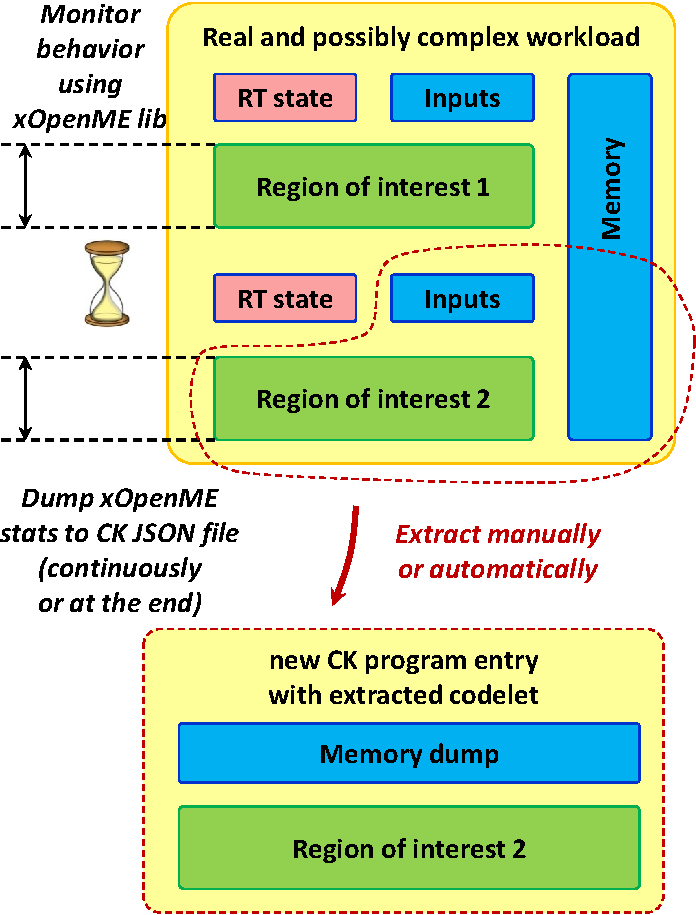
\includegraphics[width=2.5in]
      {ck-assets/1b9b091003515e71-cropped.pdf} %CK_URL={1b9b091003515e71-cropped.pdf}
     \caption{
       Preparing larger applications such as Firefox and Chrome for CK-based autotuning: 
       a) instrumenting, monitoring and optimizing hot code regions using "XOpenME" library 
       b) extracting code regions from a large application with a run-time data set and register them in the CK as standalone programs (codelets)
     }
     \label{fig:ck-codelets}
   \end{figure}

In the MILEPOST project~\cite{29db2248aba45e59:a31e374796869125} 
we used a proprietary "codelet extractor" tool from CAPS Entreprise 
(now dissolved) to automatically extract such hot spots with their data sets 
from several real software projects and 8 popular benchmark suits 
including NAS, MiBench, SPEC2000, SPEC2006, Powerstone, UTDSP and SNU-RT.
%
We shared those of them with a permissive license as CK programs 
in the \href{https://github.com/ctuning/ctuning-programs}{ctuning-programs} repository
to be compatible with the presented CK autotuning workflow.
%           
We continue adding real, open-source applications and libraries as CK program entries
(GEMM, HOG, SLAM, convolutions) or manually extracting and sharing interesting code 
regions from them with the help of the community.
%
Such a large collection of diverse and realistic workloads 
should help make computer systems research more applied and practical.

As many other scientists, we also faced a big data problem when continuously 
aggregating large amounts of raw optimization data during crowd-tuning
for further processing including machine learning~\cite{new_pub_model}.
%
We managed to solve this problem in the CK by using 
online pre-processing of raw data and online classification 
to record only the most efficient optimization solutions 
(on a frontier in case of multi-objective autotuning) 
along with unexpected behavior (bugs and numerical 
instability)~\cite{cm:29db2248aba45e59:cd11e3a188574d80}.
%
It is now possible to invoke crowd-tuning of GCC compiler flags (improving execution time) in the CK as following:
\begin{flushleft}
\texttt{\$ ck crowdtune program --iterations=50 --scenario=8289e0cf24346aa7}
\end{flushleft}

or

\begin{flushleft}
\texttt{\$ ck crowdsource program.optimization --iterations=50 --scenario=8289e0cf24346aa7}
\end{flushleft}

In contrast with traditional autotuning, CK will first query \textit{remote-ck} repository
to obtain all most efficient optimization choices aka solutions (combinations of random compiler flags in our example)
for a given trade-off scenario (GCC compiler flag tuning to minimize execution time), compiler version,
platform and OS.
%
CK will then select a random CK program (computational species),
compiler and run it with all these top optimizations,
and then try N extra random optimizations (random combinations of GCC flags) 
to continue increasing design and optimization space coverage.
%
CK will then send the highest improvements of monitored characteristics 
(execution time in our example) achieved for each optimization solution as well as worst degradations
back to a public server.
%
If a new optimization solution if also found during random autotuning,
CK will assign it a unique ID (\textit{solution\_uid} 
and will record it in a public repository.
%
At the public server side, CK will merge improvements and degradations for a given
program from a participant with a global statistics while recording how many programs 
achieved the highest improvement (best species) or worst degradation (worst species) for a given optimization
as shown in Figure~\ref{fig:ck-snapshot-of-results-gcc4}.

   % === CK crowd results GCC 4.9.2 ==================================================================
   %CK={"action":"prepare_for_latex", "cid":"slide:fdbe2cbbb5d5088e", "file":"6fa4e9181faa1385-cropped.pdf", "path":"ck-assets", "ck_image":"yes", "ck_image_width":700}
   %CK={"action":"prepare_for_latex", "cid":"slide:fdbe2cbbb5d5088e", "file":"6fa4e9181faa1385.solutions.tex", "uid":"6686449f5e795231", "path":"ck-assets"}
   %CK={"action":"prepare_for_latex", "cid":"slide:fdbe2cbbb5d5088e", "file":"6fa4e9181faa1385.solutions.html", "uid":"6686449f5e795231", "path":"ck-assets"}
   \begin{figure*}[!htbp]
     \centering
      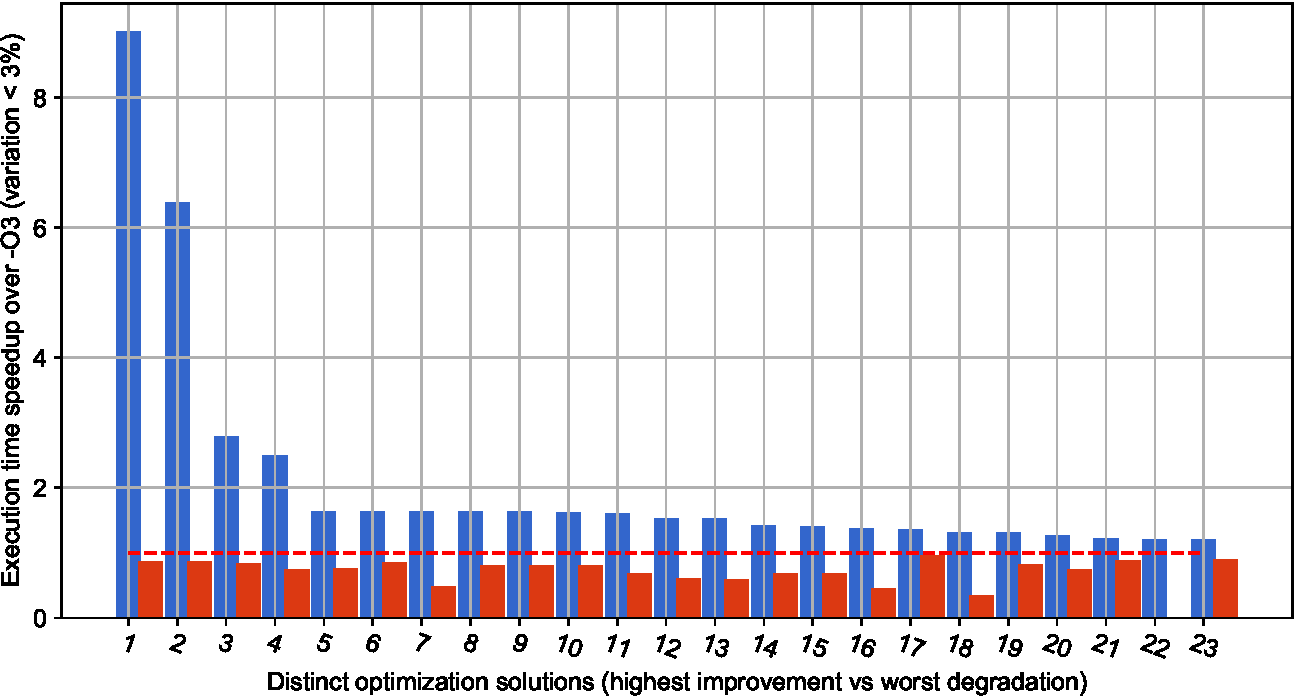
\includegraphics[width=6.0in]
       {ck-assets/6fa4e9181faa1385-cropped.pdf} %CK_URL={6fa4e9181faa1385-cropped.pdf}
      \vspace{0.1in}
          \begin{tabular}{|r|p{4.5in}|p{0.5in}|p{0.5in}|}
     \hline
     \textbf{Solution} & \textbf{Pruned flags (complexity reduction)} & \textbf{Best species} & \textbf{Worst species} \\ 
     \hline
      1 & -O3 -flto & 6 & 3 \\
     \hline
      2 & -O3 -fno-inline -flto & 1 & 1 \\
     \hline
      3 & -O3 -fno-if-conversion2 -funroll-loops & 2 & 1 \\
     \hline
      4 & -O3 -fpeel-loops -ftracer & 1 & 3 \\
     \hline
      5 & -O3 -floop-nest-optimize -fno-sched-interblock -fno-tree-copy-prop -funroll-all-loops & 4 & 1 \\
     \hline
      6 & -O3 -funroll-loops & 2 & 3 \\
     \hline
      7 & -O3 -floop-strip-mine -funroll-loops & 1 & 1 \\
     \hline
      8 & -O3 -fno-inline -fno-merge-all-constants -fno-tree-ccp -funroll-all-loops & 2 & 3 \\
     \hline
      9 & -O3 -fno-tree-loop-if-convert -funroll-all-loops & 3 & 2 \\
     \hline
      10 & -O3 -fno-section-anchors -fselective-scheduling2 -fno-tree-forwprop -funroll-all-loops & 2 & 2 \\
     \hline
      11 & -O3 -fno-ivopts -funroll-loops & 4 & 1 \\
     \hline
      12 & -O3 -fno-tree-ch -funroll-all-loops & 1 & 1 \\
     \hline
      13 & -O3 -fno-move-loop-invariants -fno-tree-ch -funroll-loops & 1 & 2 \\
     \hline
      14 & -O3 -fira-algorithm=priority -fno-ivopts & 1 & 2 \\
     \hline
      15 & -O3 -fno-ivopts & 2 & 4 \\
     \hline
      16 & -O3 -fno-sched-spec -fno-tree-ch & 1 & 2 \\
     \hline
      17 & -O3 -fno-ivopts -fselective-scheduling -fwhole-program & 1 & 1 \\
     \hline
      18 & -O3 -fno-omit-frame-pointer -fno-tree-loop-optimize & 1 & 4 \\
     \hline
      19 & -O3 -fno-auto-inc-dec -ffinite-math-only & 1 & 2 \\
     \hline
      20 & -O3 -fno-guess-branch-probability -fira-loop-pressure -fno-toplevel-reorder & 1 & 5 \\
     \hline
      21 & -O3 -fselective-scheduling2 -fno-tree-pre & 2 & 2 \\
     \hline
      22 & -O3 -fgcse-sm -fno-move-loop-invariants -fno-tree-forwprop -funroll-all-loops -fno-web & 1 & 0 \\
     \hline
      23 & -O3 -fno-schedule-insns -fselective-scheduling2 & 1 & 2 \\
     \hline
    \end{tabular} %CK_HTML={ck-assets/6fa4e9181faa1385.solutions.html}
      \vspace{0.1in}
      %CK_URL={"text":"[ Latest live results in online repository and replay info ]", "url":"http://cknowledge.org/repo/web.php?template=cknowledge&wcid=8289e0cf24346aa7:d24a4fde9f120e10"}
      %CK_INTERACTIVE_GRAPH={"action":"show","force_url":"http://cknowledge.org/repo/web.php?", "from_repo":"remote-ck","module_uoa":"experiment.tune.compiler.flags", "change_module_uoa":"8289e0cf24346aa7", "data_uoa":"d24a4fde9f120e10", "minimal":"yes", "graph_d3_div":"ck_interactive_3c4b61eebd18c00b", "remove_script_src":"yes"}
     \caption{
      Snapshot of top performing combinations of GCC 4.9.2 compiler flags together with highest speedups and worst degradations achieved across all shared CK workloads on RPi3.
     }
     \label{fig:ck-snapshot-of-results-gcc4}
   \end{figure*}


This figure shows a snapshot of public optimization results 
with top performing combinations of GCC 4.9.2 compiler flags
on RPi3 devices which minimize execution time of shared CK workloads 
(programs and data sets) in comparison with \textit{-O3} optimization level.
%
It also shows the highest speedup and the worse degradation achieved
across all CK workloads for a given optimization solution, as well
as a number of workloads where this solution was the best or the worst
(online classification of all optimization solutions).
%
Naturally this snapshot automatically generated from the public repository 
at the time of publication may slightly differ from continuously updated 
live optimization results available at this~\href{http://cknowledge.org/repo/web.php?template=cknowledge&wcid=8289e0cf24346aa7:d24a4fde9f120e10}{link}.
%
These results confirm that GCC 4.9.2 misses many optimization opportunities 
not covered by \textit{-O3} optimization level.

   % === CK crowd results GCC 7.1.0 ==================================================================
   %CK={"action":"prepare_for_latex", "cid":"slide:f07b380634136beb", "file":"41ed88477436dd3e-cropped.pdf", "path":"ck-assets", "ck_image":"yes", "ck_image_width":700}
   %CK={"action":"prepare_for_latex", "cid":"slide:f07b380634136beb", "file":"41ed88477436dd3e.solutions.tex", "uid":"a4156b772ceab9d4", "path":"ck-assets"}
   %CK={"action":"prepare_for_latex", "cid":"slide:f07b380634136beb", "file":"41ed88477436dd3e.solutions.html", "uid":"a4156b772ceab9d4", "path":"ck-assets"}
   \begin{figure*}[!htbp]
     \centering
      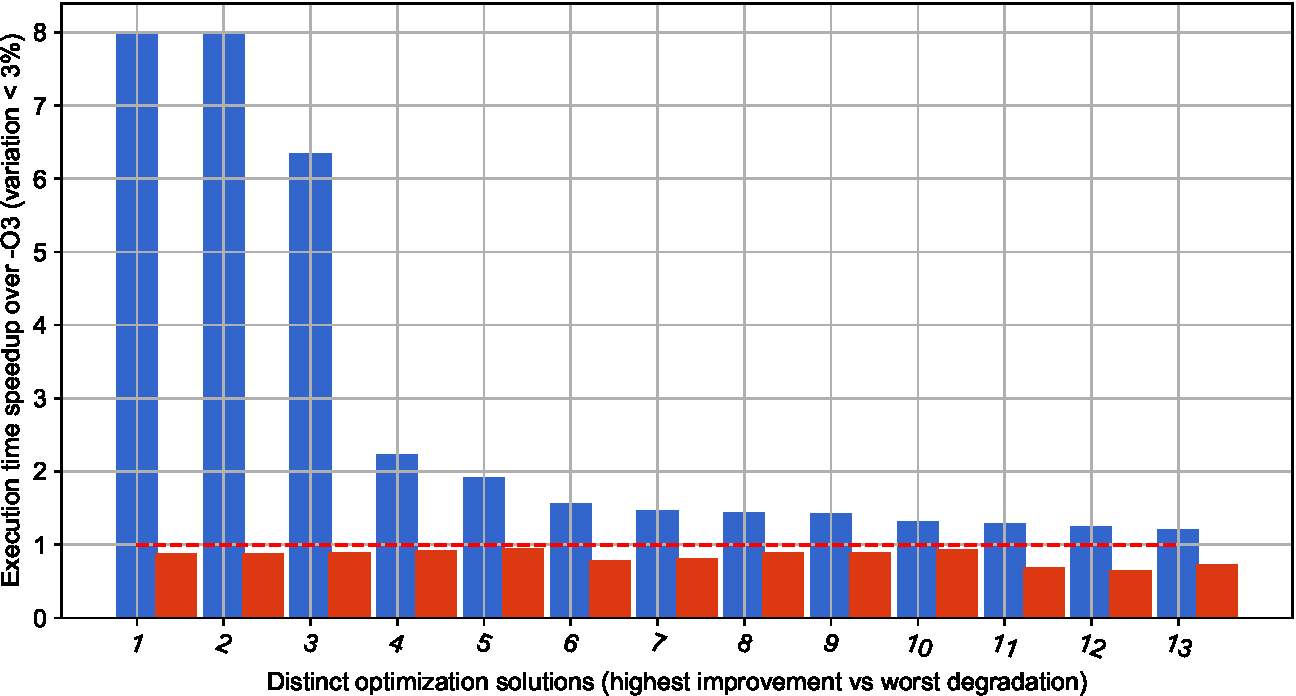
\includegraphics[width=6in]
       {ck-assets/41ed88477436dd3e-cropped.pdf} %CK_URL={41ed88477436dd3e-cropped.pdf}
      \vspace{0.1in}
          \begin{tabular}{|r|p{4.5in}|p{0.5in}|p{0.5in}|}
     \hline
     \textbf{Solution} & \textbf{Pruned flags (complexity reduction)} & \textbf{Best species} & \textbf{Worst species} \\ 
     \hline
      1 & -O3 -fno-delayed-branch -flto -fno-selective-scheduling2 -fno-whole-program & 6 & 0 \\
     \hline
      2 & -O3 -flto & 4 & 1 \\
     \hline
      3 & -O3 -fno-inline -flto & 2 & 1 \\
     \hline
      4 & -O3 -fno-cprop-registers -flto -funroll-all-loops & 3 & 1 \\
     \hline
      5 & -O3 -fno-tree-fre -funroll-all-loops & 2 & 1 \\
     \hline
      6 & -O3 -fno-predictive-commoning -fno-schedule-insns -funroll-loops & 3 & 3 \\
     \hline
      7 & -O3 -funroll-loops & 3 & 0 \\
     \hline
      8 & -O3 -fno-tree-ter -funroll-all-loops & 3 & 1 \\
     \hline
      9 & -O3 -fno-merge-all-constants -fselective-scheduling2 -funroll-loops & 1 & 0 \\
     \hline
      10 & -O3 -fno-devirtualize-at-ltrans -fno-predictive-commoning -fno-tree-pre & 1 & 2 \\
     \hline
      11 & -O3 -fcheck-data-deps -fira-loop-pressure -fno-isolate-erroneous-paths-dereference -fno-sched-dep-count-heuristic -fsection-anchors -fsemantic-interposition -fno-tree-ch -fno-tree-loop-linear -fno-tree-partial-pre & 2 & 2 \\
     \hline
      12 & -O3 -fno-schedule-insns -ftracer & 2 & 3 \\
     \hline
      13 & -O3 -fno-auto-inc-dec -fguess-branch-probability -fipa-pure-const -freorder-blocks -fselective-scheduling2 -ftree-ccp -fno-tree-pre -ftree-tail-merge & 1 & 1 \\
     \hline
    \end{tabular} %CK_HTML={ck-assets/41ed88477436dd3e.solutions.html}
      \vspace{0.1in}
      %CK_URL={"text":"[ Latest live results in online repository and replay info ]", "url":"http://cknowledge.org/repo/web.php?template=cknowledge&wcid=8289e0cf24346aa7:79bca2b76876b5c6"}
      %CK_INTERACTIVE_GRAPH={"action":"show","force_url":"http://cknowledge.org/repo/web.php?", "from_repo":"remote-ck","module_uoa":"experiment.tune.compiler.flags", "change_module_uoa":"8289e0cf24346aa7", "data_uoa":"79bca2b76876b5c6", "minimal":"yes", "graph_d3_div":"ck_interactive_1e94a8eaa9306f1e", "remove_script_src":"yes"}
     \caption{
      Snapshot of top performing combinations of GCC 7.1.0 compiler flags together with highest speedups and worst degradations achieved across all shared CK workloads on RPi3.
     }
     \label{fig:ck-snapshot-of-results-gcc7}
   \end{figure*}

Figure~\ref{fig:ck-snapshot-of-results-gcc7} with optimization results 
for GCC 7.1.0 also confirms that this version was considerably improved 
in comparison with GCC 4.9.2
(latest live results are available in our public optimization repository
at this \href{http://cknowledge.org/repo/web.php?wcid=8289e0cf24346aa7:79bca2b76876b5c6}{link}):
there are fewer efficient optimization solutions found during crowd-tuning
14 vs 23 showing the overall improvement of the \textit{-O3} optimization level.

Nevertheless, GCC 7.1.0 still misses many optimization opportunities 
simply because our long-term experience suggests that it is infeasible 
to prepare one universal and efficient optimization heuristics 
with good multi-objective trade-offs for all continuously 
evolving programs, data sets, libraries, optimizations and platforms.
%
That is why we hope that our approach of combining a common workflow framework
adaptable to software and hardware changes, public repository of optimization knowledge, 
universal and collaborative autotuning across multiple hardware platforms 
(e.g.~provided by volunteers or by HPC providers), and community involvement 
should help make optimization and testing of compilers
more automatic and sustainable~\cite{cm:29db2248aba45e59:cd11e3a188574d80,ck-date16}.
%
Rather than spending considerable amount of time on writing their own autotuning and crowd-tuning
frameworks, students and researchers can quickly reuse shared workflows, 
reproduce and learn already existing optimizations, try to improve optimization heuristics, 
and validate their results by the community. 

Furthermore, besides using \textit{-Ox} compiler levels, academic and industrial users 
can immediately take advantage of various shared optimizations solutions automatically
found by volunteers for a given compiler and hardware via CK using \textit{solution\_uid} flag.
%
For example, users can test the most efficient combination of compiler flags 
which achieved the highest speedup for GCC 7.1.0 on RPi3 
(see "Copy CID to clipboard  for a given optimization solution at this 
\href{http://cknowledge.org/repo/web.php?wcid=8289e0cf24346aa7:79bca2b76876b5c6}{link})
for their own programs using CK:

\begin{lstlisting}[breaklines]
$ ck benchmark program:{new program}
  --shared_solution_cid=27bc42ee449e880e:
  79bca2b76876b5c6-8289e0cf24346aa7-
  f49649288ab0accd
\end{lstlisting}

or

\begin{lstlisting}[breaklines]
$ ck benchmark program:{new program} 
  -O27bc42ee449e880e:79bca2b76876b5c6-
  8289e0cf24346aa7-f49649288ab0accd
\end{lstlisting}
